\documentclass{article} % For LaTeX2e
\usepackage{nips, times}
\usepackage{hyperref}
\usepackage{url}
\usepackage{graphicx}
\usepackage{amsmath}
\usepackage{amssymb}
\usepackage{booktabs}
\usepackage{tabularx}
\usepackage{caption}
\usepackage{subcaption}
\usepackage{color}
\usepackage{relsize}
\usepackage{placeins}
\usepackage{natbib}
\usepackage{paralist}
\usepackage{bbm}
\usepackage{subfigure}
\usepackage{multirow}
\usepackage{enumitem}
\usepackage[toc,page]{appendix}

\renewcommand{\null}{\operatorname{null}}
\newcommand{\given}{\,|\,}

\input math.tex

\nipsfinalcopy

\begin{document}
\title{Image Segmentation using superpixel based MRF and shape priors}

\author{
Fanny Yang\\
University of California\\
Berkeley, CA 94720, USA\\
\texttt{fanny-yang@eecs.berkeley.edu} \\
\And
Siqi Wu\\
University of California\\
Berkeley, CA 94720, USA\\
\texttt{siqi@stat.berkeley.edu}\\
}

\maketitle

\section{Introduction}
Gene expression analysis on fruitfly embryos relies on dyed images taken by a DIC microscope with generally little intensity contrast. However for each gene, a different embryo had to be used. Especially in later stages of the development the organs like mouth, gut and the yolk all lie in slightly different locations and have different shapes. In order to achieve comparability of the gene expression images one needs to map the embryos to a standard template. One way to achieve this is to segment the different organs to and derive transformations between the images and the template. 

In the problem that we try to tackle, the embryos are already considered to be aligned in a ellipse in the center of the image. The code had already been written to achieve that. Therefore one is left with the image segmentation task within the embryo, where the organs are very hard to discern even for the human eye. This is for example due to almost very little intensity variation and almost no color information.

In this paper I will outline a few commonly used image segmentation algorithms and their drawbacks when applied to the current problem. This will then lead to the motivation to propose a new algorithm which combines the different frameworks to form an algorithm which is relatively fast and accurate at the same time. The experiments are run on a toy example of separating the center embryo from other unwanted embryo parts on the border. I am aware this very example can be solved using much simpler algorithms such as ellipse fitting and edge detection, however the algorithm had to be ensured to work on this relatively simple example first before attempting to solve the original and much harder organ segmentation task.

\section{Previous works}
On a high level, the general segmentation task can be solved by minimization of an energy cost function, with each of them having an equivalent interpretation in terms of maximizing a posterior distribution. A common problem for all approaches is that they often find local structures but cannot incorporate global information. In order to overcome this, all methods also have some possibility to incorporate prior probabilities obtained by training data or prior information.

\paragraph{Deformable models}
For example, one line of method is based on the idea of Snakes \cite{Kass88_Snakes, Cootes92_ActiveShape,Cootes01_ActiveApp}, also called ``Active Contours''. The decision variable they optimize over is a parameterized contour $c(s)$ with parameterization $s$. In the simplest model, the energy consists of the length and smoothness of the curve which is the internal energy (image independent), and a term called the external energy which measures how much it is consistent with the edge image, i.e.
\beqs
E(\tilde{I},c) = E_{ext}(c) + E_{int}(I,c) = \int_0^1 \tilde{I}(c(s))\d s  + \int_0^1 \alpha(s)|c'(s)|^2 + \beta(s)|c''(s)|^2\d s
\eeqs 
where $\tilde{I}$ here is the edge image. Priors can be incorporated using point distribution models \cite{Cootes92_TrainingShape}. 

%\cite{Sclaroff01_RegionGroup, ElBaz09_ShapeApp}
% Level set 
Since the parameterization of the curve is usually cumbersome, people have proposed modelling the contour $c$ as the zero level set of a continuous function $\phi(x,y)$ \cite{Leventon00_ShapeGeodesic, ChanVese01, MumfordShah89}. There, the energy minimization decision variable is a function which thus requires techniques from functional analysis, in particular partial differential equations (PDE) such as Euler-Lagrange equations. Later, this framework was extended to enable incorporation of shape and intensity priors \cite{Cremers06_KernelDensity, Chan05_LevelShape, Chen09_LevelShapeIntensity}.

In terms of incorporating a prior, this framework allows much more flexibility and robustness since we do not need to define landmarks on a contour as in \cite{Cootes92_TrainingShape}. Furthermore, since the contour is the zero level set of a function it can detect regions with the same label which are not connected. Although this can be a desirable for certain tasks, in our particular problem of organ segmentation this is certainly an unwanted behavior.
%Bad: 

\paragraph{Graphical models}
Another line of work has concentrated on the probabilistic interpretation of energy minimization which is maximum likelihood estimation. The labels $y$ are treated as unknown variables while the image features $x$ (e.g intensity, texture etc.) are treated as observables (more details in section \ref{model}). There are mainly two different approaches: The discriminative approach (conditional random fields \cite{Lafferty01_CRFSeq, KaeSohn13_CRF}) models $p(y|x)$ directly, whereas the generative approach (Markov random fields) models $p(x|y)$ as a Gaussian distribution and uses pairwise potentials $p(y_i,y_j)$ for neighboring pixels. CRF methods generally need more training data to estimate the parameters of the distributions whereas MRF are fairly self-sufficient. 

Several unsupervised and supervised extensions have been brought forth for obtaining a globally useful segmentation using prior information such as training a hidden layer as a Restricted Boltzmann machines \cite{KaeSohn13_CRF} or multiscale representations of the feature space \cite{He04_MultiScale}. For an MRF model it is also possible to incorporate shape priors directly using a large collection of exemplars and GraphCut \cite{Lempitsky_BranchMin}. 

\paragraph{Hybrid models and superpixels}
There have already been attempts to combine the two frameworks \cite{Huang04_MRFDM, Schlesinger13}. However \cite{Huang04_MRFDM} use contour priors and \cite{Schlesinger13} require MCMC sampling which is computationally costly. Furthermore, pixelwise MRF/CRF are computationally inefficient to solve for high resolution images as in our segmentation task. In this case we exploit the work by Malik et al. \cite{Malik03_Superpixel} and pre-process the high-resolution images using the superpixel algorithm. It clusters regions according to their texture and brightness similarity as well as contour cues using trained data from natural images.
%In order to find the organs automatically we need to have a reasonably high number of superpixels such that the real contour is actually in the set of possible edges given by the superpixel edges. It should also not be too high since edges tend to become very non-smooth. 

\paragraph{Algorithms on embryo organ segmentation}
The first attempts which were made to segment the gut for example used superpixels at different scales and applied a random forest algorithm on these superpixels. Similarly a superpixel CRF and Restricted Boltzmann machines were tested on the data. However, albeit being accurate for some of the images, they could not provide a very reliable segmentation result throughout the range of different embryos. 

Since the embryos all have a similar structure for a given life stage and the superpixel segmentations usually include the desired boundary, the main idea which motivated this work is to incorporate shape priors from only few training images into the superpixel MRF framework. As we do not have a large training data set with lots of variations in the priors, the Branch-and-Bound framework proposed in \cite{Lempitsky_BranchMin} is not the most appropriate choice for our purposes. Instead we will incorporate the level set segmentation framework with shape prior into the superpixel MRF. The probability distribution over the shape priors is calculated using Gaussian kernel density estimation.

\section{Model}
\label{model}
In our novel model we use an MRF similar to the one in \cite{Huang04_MRFDM} on superpixels, however opposed to their model we do not use contours which carry the burden of pointwise parameterization, but take advantage of the level set functions. 
%Also later on we extend this framework to the super pixel level.

%We first describe the model on a pixel level. 
Let's denote $y$ as our hidden labels, $x$ as our observed superpixel features (e.g. intensities, texture, relative location etc.). We index the superpixels by $i$ and our signed distance function is $\phi(i)$. Our model for the joint probability distribution corresponds to use an undirected graphical model as in Figure \ref{figure:MRF} with node set $\Nu$ and edge set $E$. 

\begin{figure}[t]
  \centering
  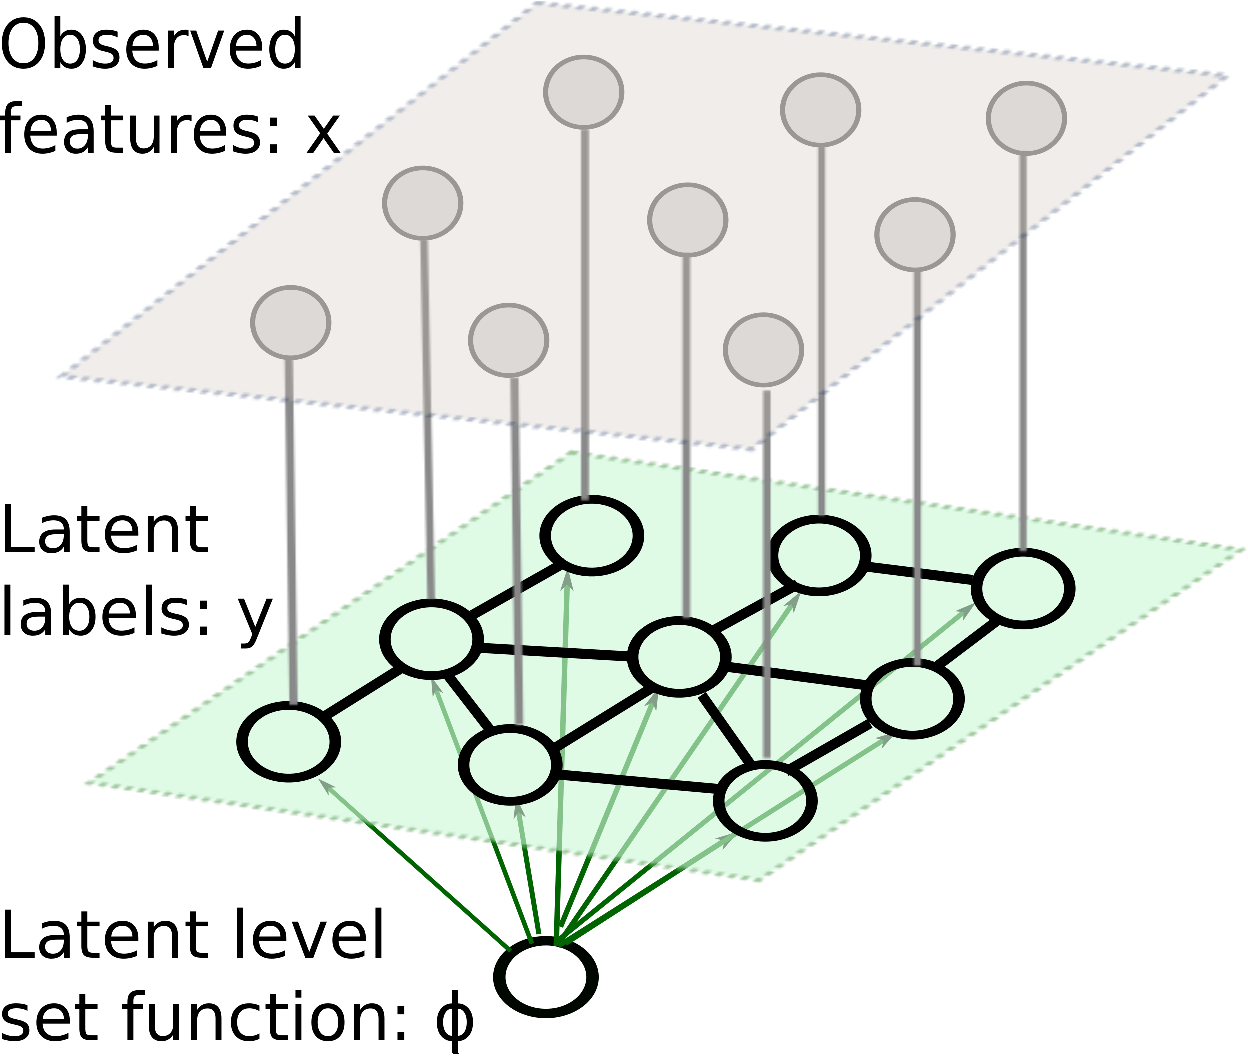
\includegraphics[scale = 0.3]{MRF.pdf}
\caption{Markov random field model}
 \label{figure:MRF}
  \end{figure}

Note that in general each superpixel can have an arbitrary number of neighbors so that the graphical model in \ref{figure:MRF} can have maximal cliques of size bigger than two. However, in our approach we only consider pairwise potentials. This leads to the following factorization
%Our graphical model, depicted in ??? allows for the following factorization with pairwise potentials $\psi$ reads
\begin{align}
p(x,y,\phi) &=  \prod_{i\in \Nu} \psi(x_i,y_i)  \prod_{(i,j)\in E} \psi(y_i,y_j)\prod_{i\in \Nu} p(y_i|\phi)p(\phi) \label{total_joint}\\
&=: \prod_{i\in \Nu} p(x_i|y_i)p(y_i,y_j)p(y_i|\phi)p(\phi|\tilde{\phi})\nonumber
\end{align}
where  $\tilde{\phi} = \{\tilde{\phi_k}\}_{k\in I}$ denote prior shapes with $I$ being the index set of shape priors.

We model $p(x_i|y_i)$ as a multivariate Gaussian mixture with means $\mu_k$ and diagonal covariance matrices $\Sigma_k$ for $k= 0,\dots,K-1$ where $K$ is the number of labels (in this paper $K=2$ for binary segmentation), i.e. 

\beqs
p(x_i|y_i = k) = \frac{1}{\sqrt{|2\pi \Sigma_k|}} \exp(-\frac{1}{2} (x- \mu_k)\Sigma_k^{-1}(x - \mu_k))
\eeqs

Our pairwise potentials penalize neighbors with different labels and read
\beq
\label{edgepot}
p(y_i,y_j) \propto \theta_1 \Indi_{y_i\neq y_j} + \theta_2 \Indi_{y_i=y_j}
\eeq

%It turns out that the choice of $\theta_i$ is best made using the observed $x_i, x_j$. 

For the consistency measure of the labels $y$ on $\phi$ we use the logistic function
\beqs
p(y_i|\phi) = \left(\frac{1}{1 + \E^{-\lambda \phi(i)}}\right)^{y_i} \left(\frac{1}{1 + \E^{\lambda \phi(i)}}\right)^{1-y_i}
\eeqs
where $\phi(i)$ is usually a signed distance function and $\lambda$ controls the sharpness of the slope. 
%Note: Schlesinger uses $\psi(y|\phi) = \E^{\sum_i y_i \phi(i)}$.

For the probability distribution on the level set function we use the well-known energy cost function \cite{Cremers06_KernelDensity, ChanVese01, MumfordShah89}
\begin{align}
p(\phi|\tilde{\phi}) &= E_{int}(\phi) + E_{prior}(\phi)\label{levelset}\\
&= \lambda_1 \int_{\Omega}\delta_\epsilon(\phi(x,y))\|\nabla \phi(x,y)\|\d x \d y + \lambda_2 \int_{\Omega}H_\epsilon(\phi(x,y))\d x \d y\nonumber\\
&- \log \sum_{i=1}^N \exp\left(-\frac{1}{2\sigma^2}d^2(H(\phi),H(\tilde{\phi}_i))\right)\nonumber
\end{align}
where $d$ is the symmetric distance between the level set functions defined as
\beqs
d^2(H_\epsilon(\phi_1),H_\epsilon(\phi_2)) = \int_{\Omega} (H_\epsilon(\phi_1) - H_\epsilon(\phi_2))^2 \d x\d y
\eeqs
Instead of using the non-differentiable Heaviside function we apply a smoothed version, i.e. 
\beqs
H_\epsilon(z) = \frac{1}{2}(1+ \frac{2}{\pi}\arctan \left( \frac{z}{\epsilon} \right))
\eeqs
as in \cite{ChanVese01} with derivative $\delta_\epsilon(z) = \frac{\epsilon}{z^2 + \epsilon^2}$. The $\epsilon$ is dropped in the following for simpler notation.

$E_{int}$ denotes the regularization on length and area of the region (boundary), $E_{prior}$ is the energy given by the shape prior which gives the probability of $\phi$ given the training data set $\tilde{\phi}$. The shape distribution is estimated using nonparametric kernels with width $\sigma^2=\frac{1}{N}\sum_{i=1}^N \min_{j\neq i}d^2(H(\phi_i),H(\phi_j))$.
% is measured as a distance $d^2(H(\phi),H(\phi_i)) = \int_{\Omega}(H(\phi)-H(\phi_i))^2\d x$ is basically doing a nonparametric kernel density estimation for the shape distribution using given samples $\phi_i$. We choose for the kernel width $\sigma^2=\frac{1}{N}\sum_{i=1}^N \min_{j\neq i}d^2(H(\phi_i),H(\phi_j))$.


\subsection{Variational inference approach}
The inference task now is to maximize $p(y,\phi|x) \propto p(x,y,\phi)$. However finding the maximum of \eqref{total_joint} exactly is computationally intractable. First of all the graphical model is not a tree and secondly the domain of $\phi$ is infinite dimensional. A very nice framework to overcome this difficulty is to use shape priors directly in the model as described in \cite{Lempitsky_BranchMin} since submodular quadratic pseudo-boolean function of the form
\beqs
E(y) = a + \sum_i a_i y_i + \sum_{i,j}a_{ij}y_i y_j
\eeqs
can be computationally efficiently. However as mentioned above their approach for incorporating priors is not suitable for our task and the general GraphCut approach does not work for infinite dimensional variables. The aim is thus to approximate the conditional distribution by adding variational parameters $a,b$ which render the labels and the level set function conditionally independent. 

%% These maximum likelihood problems are generally impossible to solve exactly since the graphical model is not a tree so that one has to use loopy belief propagation or variational inference methods (???). However for binary segmentation the GraphCut algorithm for example (???) is able to solve the problem precisely under the condition that the cost function is a submodular quadratic pseudo-boolean function of the form
%% \beqs
%% E(y) = a + \sum_i a_i y_i + \sum_{i,j}a_{ij}y_i y_j
%% \eeqs
%% where $y_i\in {0,1}$ for each $i$ and possibly depend on the observations $x$. 


This approach is called variational inference \cite{Jordan99_Variational, Wainwright_Variational} and our ansatz for the structure of $Q$ is the following factorization
\beq
\label{VariationalAnsatz}
Q(y,\phi|x,a,b) = Q_M(y|x,a)Q_D(\phi|b) 
\eeq
with $Q_M(y|x,a) = \prod_{i,j} \psi(y_i,y_j) \prod_i  \xi(x_i,y_i) p(y_i|a_i)$ and $Q_D(\phi|b) \propto \prod_i p(b_i|\phi) p(\phi)$. 
The best approximation $Q$ with this structure is found by minimizing the Kullback Leibler divergence $KL(Q||P) = \sum_\phi \sum_y Q(y,\phi|x,a,b) \log \frac{Q(y,\phi|x,a,b)}{p(y,\phi|x)}$ over $a$ and $b$. 

%% Our ansatz for the structure of $Q$ is the following factorization
%% \beqs
%% Q(y,\phi|x,a,b) = Q_M(y|x,a)Q_D(\phi|b) 
%% \eeqs
%% with $Q_M(y|x,a) = \prod_{i,j} \psi(y_i,y_j) \prod_i  \xi(x_i,y_i) p(y_i|a_i)$ and $Q_D(\phi|b) \propto \prod_i p(b_i|\phi) p(\phi)$ so that we have factorized the distribution with respect to the two unknown vectors $y, \phi$. We are hence assuming independence of the two, given $a,b$ respectively.

Using this factorization the KL divergence can be rewritten as
\begin{align*}
KL(Q||P) &=\EE \log Q_M(y|x,a) + \EE \log Q_D(\phi|b) - \EE \log p(y,\phi|x)\\
 &=\EE \left[\log Q_M(y|x,a)|\phi \right] + \EE \left[ \log Q_D(\phi|b) |y\right] - \EE \left[\EE \log p(y|\phi) |\phi \right]- \EE \log p(\phi)\\
 &=\EE_{Q_M} \left[\log Q_M(y|x,a) - \EE_{Q_D} \log p(y|\phi)\right] + \EE_{Q_D} (\log Q_D(\phi|b) - \log p(\phi))%\\
%= &\EE_{Q_M} (\log Q_M(y|x,a) - \EE_{Q_D} \log p(y|\phi)) + \EE_{Q_D} (\log p(b|\phi) + c)
\end{align*}
where $c$ is a constant independent of $a$ and $b$. The first equality follows from the conditional independence of $y,\phi$ given $a,b$.% and the second uses $Q_D(\phi) = p(\phi)$.

For the minimization of this term with respect to $a,b$ we use Lagrange equations of first kind to incorporate the constraint of $\EE \left[Q_D(\phi|b) |b \right] = 1$ and $\EE \left[ Q_M(y|x,a) |x,a\right] = 1$ and obtain for the Lagrange multiplier $\lambda = 1$. Then we set the partial derivatives with respect to the distributions to zero 
% --------- Add for Group report!
\begin{align*}
\frac{\partial \L}{\partial Q_M} &= -\EE_{Q_D} \log p(y|\phi) + \log Q_M(y|x,a) = 0\\
\implies  &\sum_i (\EE_{Q_D}\log p(y_i|\phi) - \log p(y_i|a_i)) = \sum_{j\in N(i)} \log p(y_i,y_j) - \EE_{Q_D} \log(p(y_i,y_j)) \\
\frac{\partial \L}{\partial Q_D}&=  - \EE_{Q_M} \log p(y|\phi) + \log p(b|\phi) = 0
\end{align*}
% -----------------------------------
from which it follows that the following fixed point equations must hold for optimal $a,b$:
\begin{equation}
\label{fixedpoint}
\log p(y_i|a_i) = \EE_{Q_D} \log p(y_i|\phi),\qquad \log p(b_i|\phi) &= \EE_{Q^i_M} \log p(y_i|\phi) 
\end{equation}
where $Q_M^i = Q_M(y_i|x,a)$.



\section{Algorithm}
The algorithm now has to find $p(y_i|a_i)$, $p(b_i|\phi)$ and $\phi$ which satisfy \eqref{fixedpoint} before maximizing $Q$ as in \eqref{VariationalAnsatz}. This is done by using a non-informative initialization for $p(y_i|a_i)$ and an alternating minimization approach for the update steps. Instead of using \eqref{fixedpoint} in its exact form, we approximate $Q_D(\phi|b)$ by a dirac distribution $Q_{D'}(\phi|b) = \delta_{\phi = \phi^*}$ where $\phi^* = \argmax_{\phi} Q_D(\phi|b)$ is found by running a level set segmentation algorithm. Then the conditional probability reads
\beq
\label{approximatep}
p(y_i|a_i) \approx \exp(\EE_{Q'_D} \log p(y_i|a_i)) =  p(y_i|\phi^*)
\eeq
Given $p(y_i|a_i)$ we can calculate $Q_M(y_i|x_i,a)$ by estimating the parameters for $p(x_i|y_i)$ using the EM algorithm. At the same time we are interested in $Q_M(y_i|x,a)$ for computing $p(b_i|\phi)$ for which we need to compute the marginal. Since it is not a tree, we cannot obtain the exact marginal via simple message passing but have to rely on loopy belief propagation or other alternative approximate inference methods. In fact, as will be seen in section \ref{EMalgo}, the marginalization will have to be computed as the E-Step of the EM algorithm. 

The algorithm now executes the following steps
\begin{itemize}
\item Initialize $p(y_i|a_i)$ by a uniform distribution.
\item Step $k$.
\begin{enumerate}
\item In order to calculate $Q_M(y_i|x_i,a)$ estimate the parameters $\mu_k,\Sigma_k$ of $p(x_i|y_i)$ %(which are $\mu_k,\Sigma_k$) using the EM algorithm %latent variable $y_i$ and the EM algorithm
\item Given $Q_M(y_i|x_i,a)$ use approximate inference methods to compute $Q_M(y_i|x,a)$.
% loopy belief propagation/mean field inference to obtain .
\item Calculate $\log p(b_i|\phi) = \EE_{Q_M^i} \log p(y_i|\phi)$.
\item Calculate $\phi^* = \argmax_{\phi} Q_D(\phi|b)$ using \eqref{levelset_update} and obtain $p(y_i|a_i)$ as in \eqref{approximatep}
\end{enumerate} 
\item Upon termination: $y_i = \max_k Q_M(y_i = k|x,a)$ which will have already been solved in step 2.
\end{itemize}
In the following the different steps in the algorithm will be elaborated in more detail.

\subsection{EM algorithm using loopy belief propagation}
\label{EMalgo}

In the first step, we need to estimate the parameters for $p(x_i|y_i)$ by maximizing the log likelihood $\log p(x|\theta,a) = \log \sum_y p(x|y,\theta)p(y|a)$ with respect to $\theta$ which is the same as
\beqs
\max_\theta \log p(x|\theta,a)  \propto \max_\theta \log \sum_y Q_M(y|x,a)
\eeqs

This is a classical case to employ the EM algorithm. 
Note that 
\begin{align*}
\L(q^{(t+1)},\theta) &= \sum_y Q_M(y|x,\theta^{(t)}) (\log p(x|y,\theta) + \log p(y|a)) \\
&= \sum_i \sum_{y_i} \log p(x_i|y_i,\theta) \sum_{y_j:j\neq i} Q_M(y|x,\theta^{(t)},a) + c\\
% -----------  Add for group report!
 &= \sum_i \sum_{y_i} Q_M(y_i|x, \theta^{(t)},a) \Indi_{y_i=l} (-\log \sigma_l - \frac{(x_i -\mu_l)^2}{2\sigma_l^2}) + c\\
% ----------------------------------------
&= \sum_i \sum_l Q_M(y_i = l|x,\theta^{(t)},a) (-\log \sigma_l -  \frac{(x_i -\mu_l)^2}{2\sigma_l^2}) + c
\end{align*}
where $c$ is independent of $\theta$. Thus for the expectation step we need to compute the marginal
\beqs
Q_M(y_i|x,\theta^{(t)},a) \propto \sum_{y_j:j\neq i} \prod_i p(x_i|y_i) \prod_{i,j} p(y_i,y_j) \prod_i p(y_i|a_i)
\eeqs
 given the current parameter estimates which is used in step 3 of the algorithm.

For the maximization step we maximize $\L(q^{(t+1)},\theta)$ over $\theta$ which yields
\begin{align*}
\mu_k^{(t+1)} &= \frac{\sum_i Q_M(y_i=k|x,\theta^{(t)},a) x_i}{\sum_i Q_M(y_i=k|x,\theta^{(t)})}\\
\Sigma_k^{(t+1)} &= \frac{\sum_i Q_M(y_i =k | x,\theta^{(t)},a)(x_i-\mu_k^{t+1})(x_i-\mu_k^{t+1})^T}{\sum_i Q_M(y_i = l|x,\theta^{(t)},a)}
\end{align*}
for $k = 0,\dots,K-1$.
% which intuitively just computes the average and variance of the feature within one label.


%% We write down the complete likelihood
%% \beqs
%% p(x_i|\theta_i) = p(y_i=1|a_i)p(x_i|y_i=1,\theta_1) + p(y_i=0|a_i)p(x_i|y_i=0,\theta_0)
%% \eeqs
%% We need to maximize this likelihood. 


\subsection{Level Set Segmentation with prior coupled with MRF}
\label{levelset}
In this section we will briefly sketch the classical level set segmentation approach which we will then augment by the coupling with the MRF. In general the task is to maximize $p(x,\phi) = p(x|\phi)p(\phi)$ with observed $x$ with respect to $\phi$. The term $p(\phi)$ enables us to incorporate priors and regularizations.  Note that instead of $p(x|\phi)$ in level set formulations we now have $p(y,\phi)$, or in our variational inference framework $Q_D(\phi|b) \propto p(b|\phi)p(\phi|\tilde{\phi})$.

In order to maximize 
\beqs
Q_D(\phi|b) = p(b|\phi)p(\phi) =  \exp(\left-(E_{int}(\phi)+E_{prior}(\phi,\tilde{\phi}) + E_{MRF}(\phi,Q_M))\right)
\eeqs
which is the same as minimizing the energies $E_{int}, E_{prior}$ as in \eqref{levelset} and $E_{MRF} =  \EE_{Q_M^i}\frac{\partial}{\partial \phi}\log p(y_i|\phi)$, we use the multivariate Euler Lagrange equations \cite{Evans_PDE}. They state that $F(x) = \int \L(x,\phi(x),\nabla \phi(x))\d x$ is minimized if 
% for which Euler-Lagrange equation for multivariates $x$ yields the following fixed point equation for the optimal $\phi^*$:
\beqs
\frac{\partial}{\partial \phi} \L(x,\phi(x),\nabla \phi(x))  + \divop \frac{\partial}{\partial \nabla \phi} \L(x,\phi(x),\nabla \phi(x))=0
\eeqs 
In words, $E_{MRF}$ is the term which couples the MRF and level segmentation framework.

%% We now add time for the evolution of the function and minimize the energy with respect to $\phi$ using the update equation
In order to find the $\phi$ which solves this equation we initialize the level set function and perform gradient steps obeying
\begin{align}
\frac{\partial \phi}{\partial t} = &-\frac{\partial E_{int}(\phi)}{\partial \phi} - \frac{\partial E_{prior}(\phi)}{\partial \phi} + \EE_{Q_M^i}\frac{\partial}{\partial \phi}\log p(y_i|\phi) \label{levelset_update}\\
=  & \delta_{\epsilon}(\phi) (\lambda_1 \left[\divop(\frac{\nabla \phi}{\|\nabla \phi\|})\right] +\lambda_2) - \frac{\sum_{i\in I} \alpha_i \frac{\partial}{\partial \phi} d^2(H(\phi),H(\tilde{\phi}_i))}{2\sigma^2 \sum_i \alpha_i}\nonumber\\
&+\EE_{Q_M^i} \lambda\left(\frac{y_i}{1 +\E^{\lambda \phi}} - \frac{1-y_i}{1 + \E^{-\lambda \phi}}\right)\nonumber
\end{align}
with $\alpha_i = \exp(-\frac{d^2(H\phi,H\phi_i)}{2\sigma^2})$.
%This is basically doing a gradient descent. 
For the second term, since $E_{prior}$ is a direct function of $\phi$, we can readily take the partial derivative with respect to $\phi$. $\frac{\partial}{\partial \phi} d^2(H(\phi),H(\phi_i))}
$ is a Gateaux derivative and yields
\beqs
\frac{\partial}{\partial \phi} d^2(H(\phi),H(\tilde{\phi}_i)) = \delta_{\epsilon}(\phi)(H(\phi)-H(\tilde{\phi}_i))
\eeqs

The continuous first term in \eqref{labelset_update} can be expanded to
\beqs
\divop \frac{\nabla \phi}{\|\nabla \phi\|} = \frac{ \frac{\partial^2 \phi}{\partial x^2} (\frac{\partial \phi}{\partial y})^2 - 2 \frac{\partial^2 \phi}{\partial x \partial y} \frac{\partial \phi}{\partial x}\frac{\partial \phi}{\partial y} +  \frac{\partial^2 \phi}{\partial y^2} (\frac{\partial \phi}{\partial x})^2}{(\frac{\partial \phi}{\partial x}^2  + \frac{\partial \phi}{\partial y}^2)^{\frac{3}{2}}}
\eeqs
which we implement in our algorithm using finite differences.

%% In our implementation we simply approximate the continuous derivatives by finite differences (this is exactly the formula they use in the Chan Vese Matlab package).

%% The overall formula for the update thus reads
%% \begin{align*}
%% \frac{\partial \phi}{\partial t} &= \delta_{\epsilon}(\phi)(\lambda_1  \frac{ \frac{\partial^2 \phi}{\partial x^2} (\frac{\partial \phi}{\partial y})^2 - 2 \frac{\partial^2 \phi}{\partial x \partial y} \frac{\partial \phi}{\partial x}\frac{\partial \phi}{\partial y} +  \frac{\partial^2 \phi}{\partial y^2} (\frac{\partial \phi}{\partial x})^2}{(\frac{\partial \phi}{\partial x}^2  + \frac{\partial \
%% phi}{\partial y}^2)^{\frac{3}{2}}} + \lambda_2) \\
%% &- \frac{\sum_i \alpha_i  \delta_{\epsilon}(\phi)(H(\phi)-H(\phi_i))}{2\sigma^2 \sum_i \alpha_i}\nonumber
%% \end{align*}


%% \subsection{Combining MRF with level set segmentation}
%% Rather than only 
%% The coupling of the two frameworks happens in the step when we calculate the minimum of
%% \beqs
%% -\log Q_D(\phi|b) = -\log p(b|\phi) - \log p(\phi) = - \log p(\phi) - \EE_{Q_M^i}\log p(y_i|\phi)
%% \eeqs
%% We can use our results derived in section \ref{levelset} and arrive at the update step
%% \begin{align*}
%% \frac{\partial \phi}{\partial t} &= \frac{\partial}{\partial \phi} \log p(\phi) +\EE_{Q_M^i} \frac{\partial}{\partial \phi} \log p(y_i|\phi)\\
%% &= \delta_{\epsilon}(\phi)(\lambda_1  \frac{ \frac{\partial^2 \phi}{\partial x^2} (\frac{\partial \phi}{\partial y})^2 - 2 \frac{\partial^2 \phi}{\partial x \partial y} \frac{\partial \phi}{\partial x}\frac{\partial \phi}{\partial y} +  \frac{\partial^2 \phi}{\partial y^2} (\frac{\partial \phi}{\partial x})^2}{(\frac{\partial \phi}{\partial x}^2  + \frac{\partial \phi}{\partial y}^2)^{\frac{3}{2}}} + \lambda_2) \\
%% &- \frac{\sum_i \alpha_i  \delta_{\epsilon}(\phi)(H(\phi)-H(\phi_i)}{2\sigma^2 \sum_i \alpha_i} + \EE_{Q_M^i} \lambda(\frac{y_i}{1 +\E^{\lambda \phi}} - \frac{1-y_i}{1 + \E^{-\lambda \phi}})
%% \nonumber
%% \end{align*}

%% \begin{equation}
%% \label{combined_update}
%% \frac{\partial \phi}{\partial t} = -\frac{\partial E_{int}(\phi)}{\partial \phi} - \frac{\partial E_{prior}(\phi)}{\partial \phi}  -  \EE_{Q_M^i}\frac{\partial}{\partial \phi}\log p(y_i|\phi)
%% \end{equation}


%% \subsection{On a superpixel level}
%% In the case of superpixels we use the same MRF as above, however we do not have a perfect lattice structure anymore which had directly corresponded to the pairwise potentials. Nevertheless we stick to the same probability distribution model as in - which could be more correctly modeled by a factor graph. ... ???

%% Instead of pixel intensities we use the mean and standard deviation of the intensities within the superpixels and model 
%% \beqs
%% p(\bx_i|y_i = k) = \frac{1}{2\pi \sqrt{|\Sigma_k|}} \exp(-\frac{1}{2} (\bx- \mathbf{\mu}_k)\Sigma_k^{-1}(\bx - \mathbf{\mu}_k))
%% \eeqs



\section{Implementation and Results on a toy example}

\subsection{Toy Example Setting}
For a much simpler example than organ segmentation to test our algorithmic framework, we have chosen the following problem: The task is to find the exact boundary of the center embryo in an image where parts of other embryos are sticking in and might actually share boundaries with the embryo of interest. The aim is to automatically find the boundary with only little training data.

In the results shown below, a total of 3 training images (from touching and non-touching embryos) was used for the shape priors, where each embryo was segmented manually and its shape shifted and resized leading to a pool of 27 priors in total.

\subsection{Implementation details}
We set the number of desired superpixels to 50. For building the edge structure after running the superpixel algorithm, we add an edge between two superpixels if their common boundary is above a certain length. We also merge very small superpixels if their number of pixels is below a threshold of 100. 

The smoothing constant $\epsilon$ in the Heaviside function was chosen to be $10$ and $\lambda_2 =0$ for simplicity. %Also prone to constant choices of e.g. $\lambda$ in $p(y_i|\phi)$. 
For all studied cases $\lambda_1 = 5$ yielded a good result.  In order to overcome numerical issues (since the exponential rendered all values even of $d^2/\sigma^2 \sim 100$ to zero) the kernel width $\sigma$ also had to be chosen as $\sigma^2 = \max_i d^2(H(\phi),H(\tilde{\phi}_i))$. The level set segmentation part of the algorithm was iterated for a fixed number of 100.

As features of the superpixels we choose the intensity mean and standard deviation. For the edge potential we use information about the probability boundary (which the probability of each pixel to be an edge and is also computed as a side product in the superpixel algorithm) in the following way in \eqref{edgepot}
\beqs
\theta_2 = 1 - \tilde{e}(i,j)+ \epsilon, \: \theta_1 = 1
\eeqs
where $\tilde{e}(i,j)$ is the normalized average probability along the boundary between superpixel $i$ and $j$.


In order to speed up computation we run the superpixel algorithm on a rescaled image (by $30\%$) and apply the level set segmentation with shape prior on an even smaller scale (in this example case $7\%$). This way we can make use of the sophisticated superpixel algorithm to encode high resolution information in the feature representation of the superpixels and run both MRF and level set segmentation efficiently in much smaller dimensions.

For all of the 9 test pictures, the algorithm is found to converge after less than 4 iterations. For each picture that amounts to at most 60 seconds on a ThinkPad, including running the super pixel algorithm, which is the computationally most expensive and takes 35 seconds on its own.


\subsection{Results and Discussion}

An example of an original image of touching embryos is shown in Figure \ref{Superpixels}(a). One can see how the shared boundary of the two embryos is fairly long which makes the separation harder.
The superpixel algorithm gives the pre-segmentation and edge structure depicted in Figure \ref{Superpixels}(b). As mentioned before one can observe that the ultimate correct boundary of the center embryo is correctly ``found'' by the superpixel algorithm and edges are only added if the shared boundary between two superpixels is long enough.

 \begin{figure}[htbp]
  \centering
  \subfigure[]{
  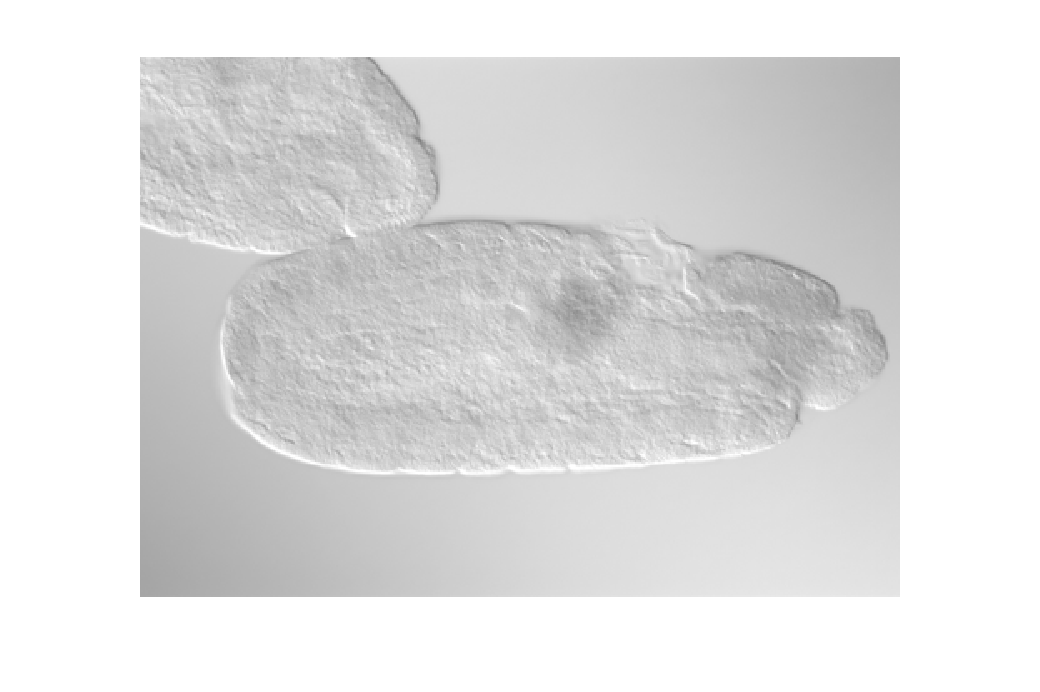
\includegraphics[scale=0.3]{touching2.pdf}
  }
  \subfigure[]{
  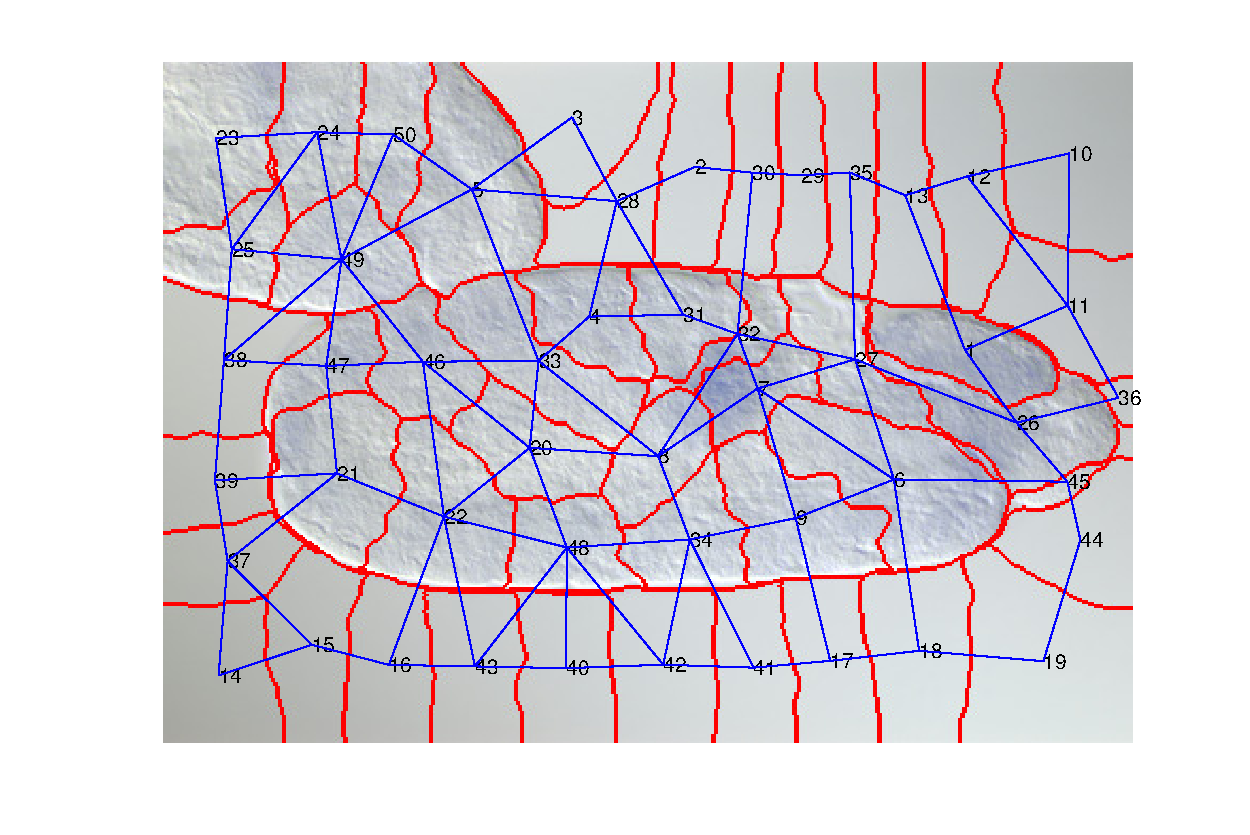
\includegraphics[scale=0.25]{fruitflyEmbSuperPixelEg.pdf}
 }  
\caption{(a) Original picture. (b) Superpixel segmentation with edge structure for MRF (on a resized image)}
\label{Superpixels}
 \end{figure}

We now show some results of the proposed algorithm. We first compare the algorithm on a test set with the individual approaches in Figure \eqref{Individualresults}. The superpixel MRF approach directly applied on the superpixel level detects both embryos as the object of interest since they are distinct from the homogeneous background. The level set segmentation alone concentrates around areas with dark intensity but misses the global structure. Adding the prior term as in \cite{Cremers06_KernelDensity} adds global structure but it still cannot find the exact edges (see also Figure \ref{MRFvsCV}). Another problem is that it is much harder to balance between the influence of the shape prior and the image given intensity cues. 

% ----------- Add to group report
Note that this picture sh/could be in case because of too strong shape prior.
% -----------------------------
These issues can be resolved by combining the advantages of  all three approaches to find the perfect contour in Figure \ref{Individualresults}(d). The pixelation of the contour is due to the image resizing for computational efficiency.

 \begin{figure}[htbp]
  \centering
  \subfigure[]{
  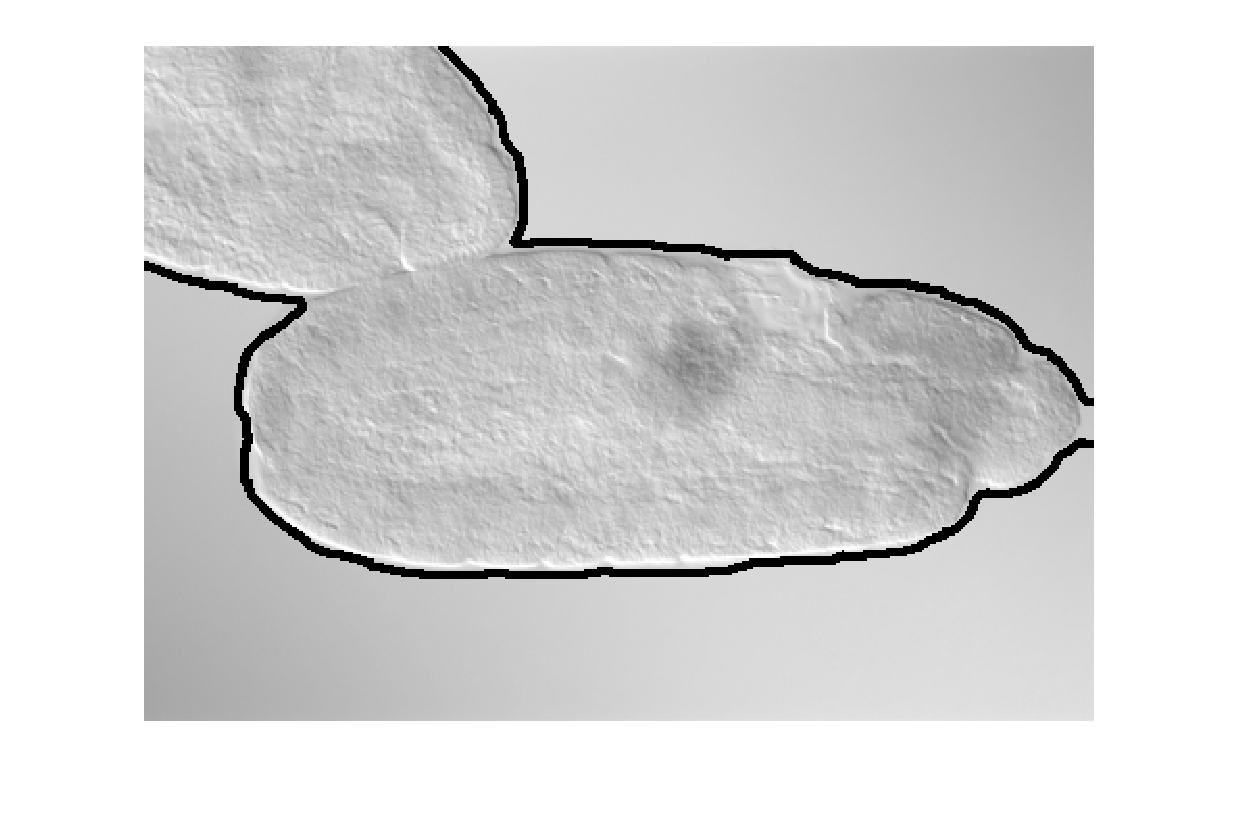
\includegraphics[scale=0.25]{MRFtouching2.pdf}
  }
  \subfigure[]{
  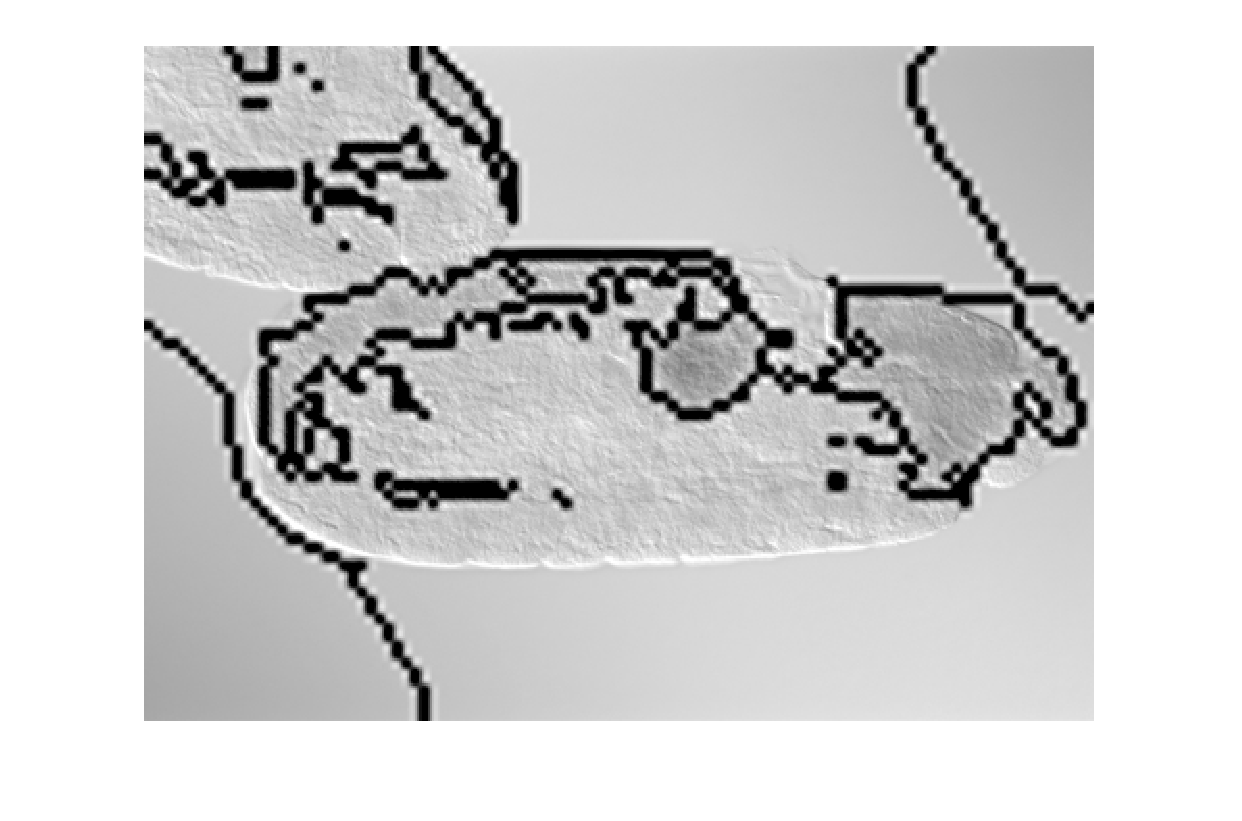
\includegraphics[scale=0.25]{CVtouching2.pdf}
 }  
\subfigure[]{
  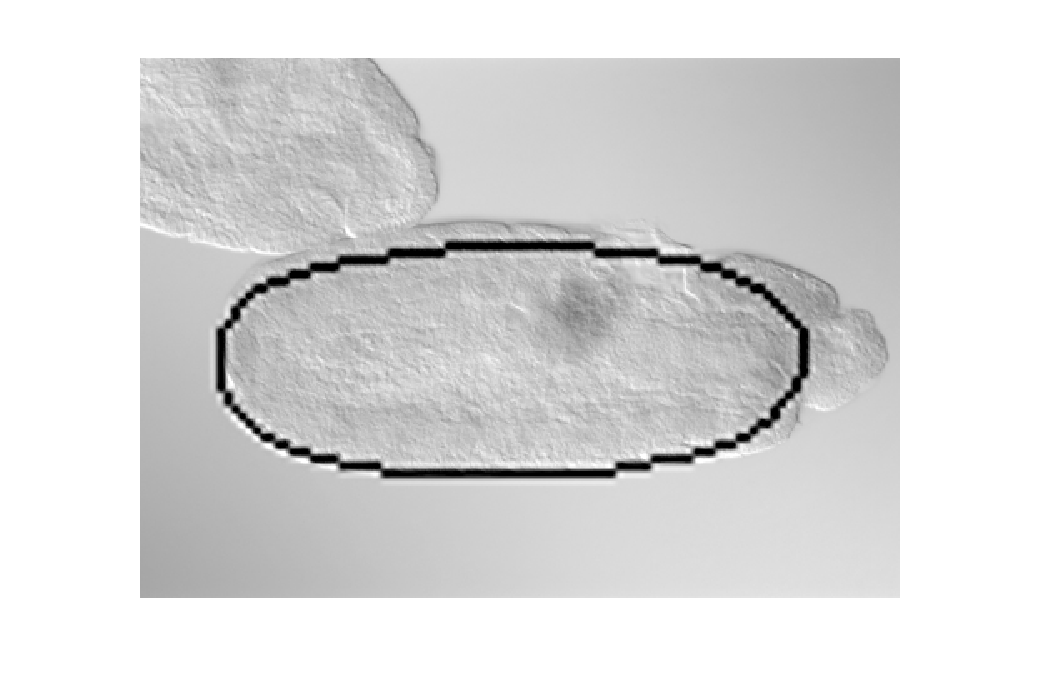
\includegraphics[scale=0.3]{MRFCVtouching2.pdf}
 }  
  \subfigure[]{
    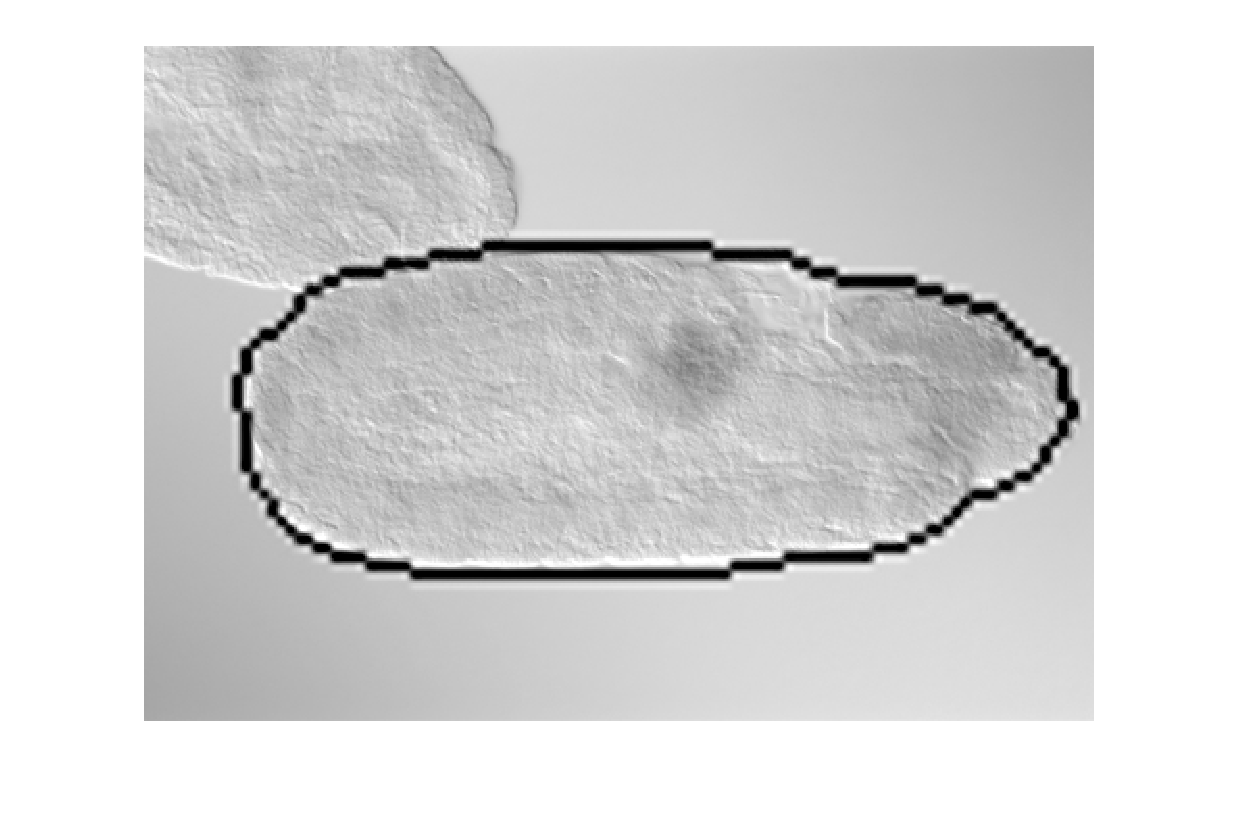
\includegraphics[scale=0.25]{hybridPriorTouching2.pdf}
  }
\caption{(a)  MRF on superpixels. (b) Level set segmentation. (c) Level set segmentation and prior.  (d) MRF with level set segmentation}
\label{Individualresults}
 \end{figure}

All of the depicted results are obtained by the mean field maximum likelihood inference on the Markov random field. An interesting observation is that the level set segmentation does not always find the boundary entirely correctly, i.e. the set $\{i\in \Nu: \phi(i) >=0\}$  does not entirely match with the set $\{i\in \Nu: y_i =1\}$ found by the MRF maximum likelihood. 
\begin{figure}[htbp]
\centering
\subfigure[]{
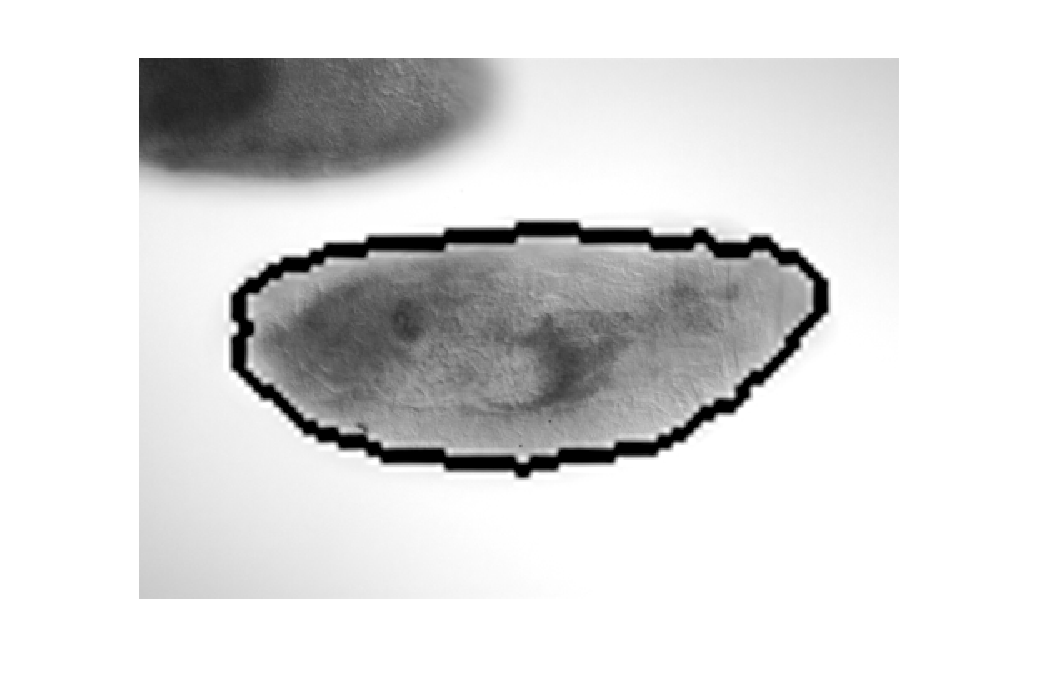
\includegraphics[scale=0.4]{MRFTouching8.pdf}
}
\subfigure[]{
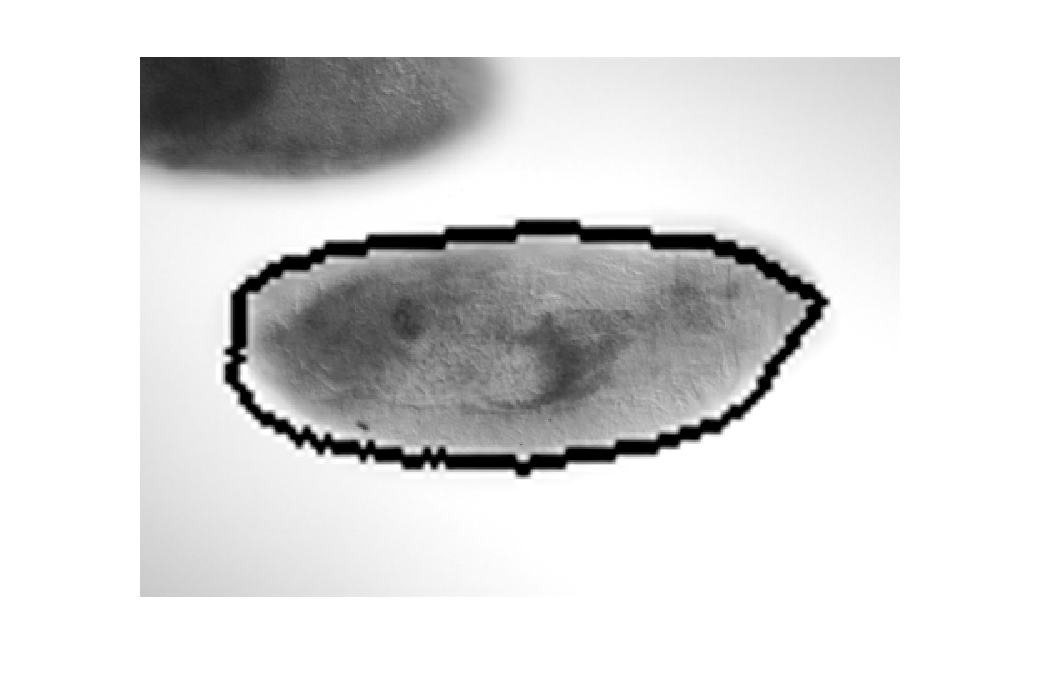
\includegraphics[scale=0.4]{CVTouching8.pdf}
}
\caption{(a) shows the final result found by the MRF, (b) depicts the zero level set found by the level set segmentation algorithm}
\label{MRFvsCV}
\end{figure}

In Figure \ref{ResultsTraining} and \ref{ResultsTest} we show results of our algorithm on our test and training images. In most of the cases, the edges can be found very precisely. In practice it turned out that the choice of the constant $\lambda_1$ needs to be carefully tuned, as it determines the influence of the MRF on the level set segmentation which should neither be too strong such that the shape prior distribution can ``drive'' the contour to the center, nor too small such that the level set algorithm does not get stuck on the ``mean'' prior. However the coupled model is much more robust to inappropriate choices of the constant as we observe that the set $\{i\in \Nu: \phi(i) >=0\}$  does not always entirely match with the set $\{i\in \Nu: y_i =1\}$ found by the mean field inference on the Markov random field. In fact, all results shown in Figures \ref{ResultsTest} are obtained by the MRF. In practice this means that if the level set segmentation does not find the perfect edge e.g. because of too strong priors, there is a chance that the superpixels will use the high-resolution information to yield the correct result.

\begin{figure}[htbp]
\centering
\subfigure{
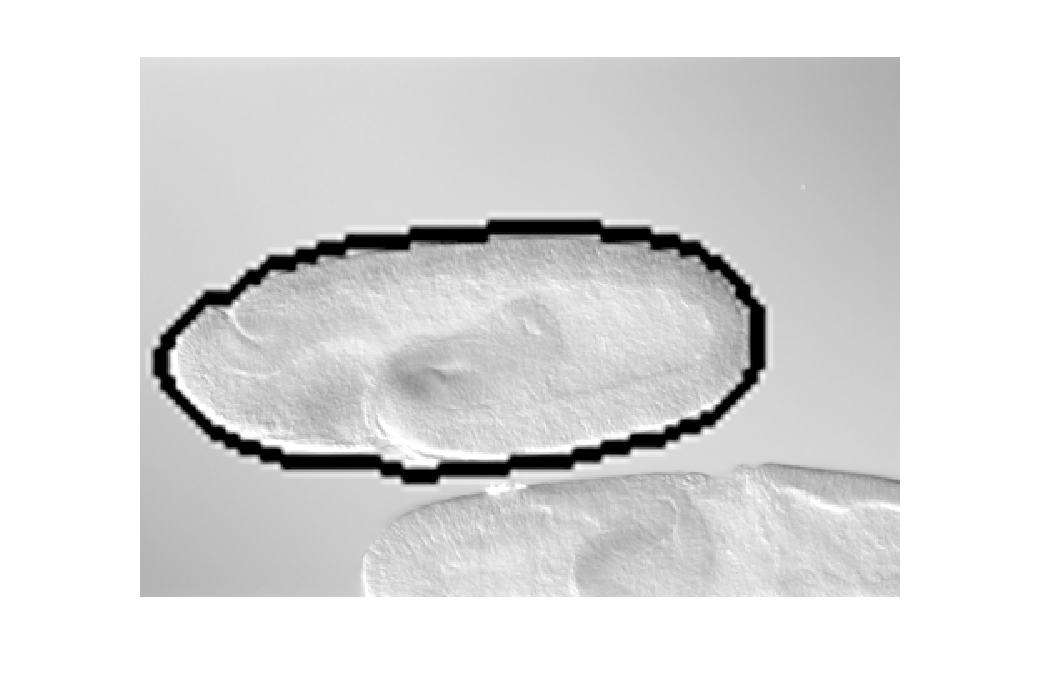
\includegraphics[scale=0.25]{hybridPriorTouching1.pdf}
}
\subfigure{
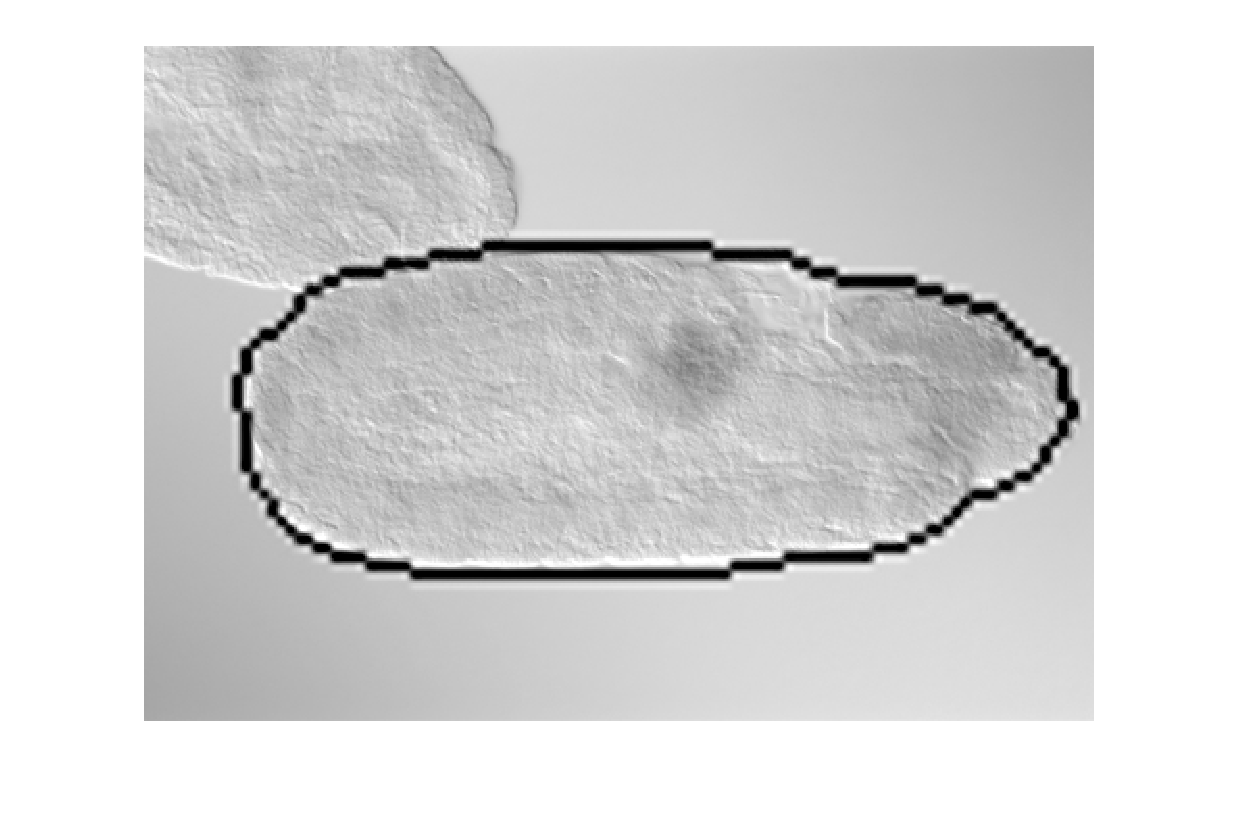
\includegraphics[scale=0.2]{hybridPriorTouching2.pdf}
}
\subfigure{
  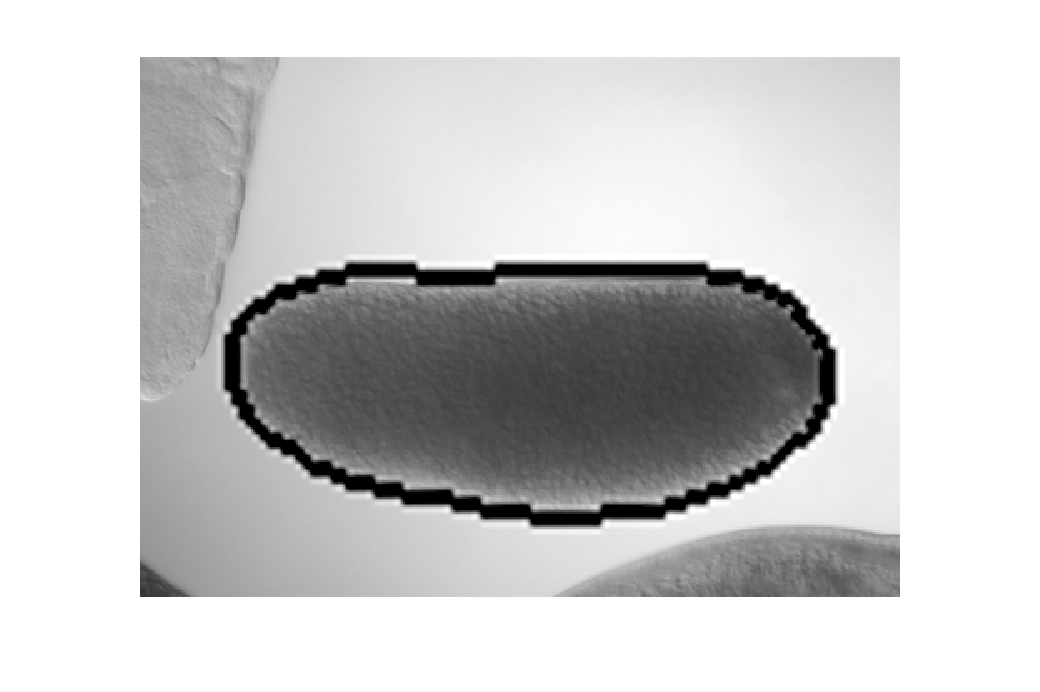
\includegraphics[scale=0.25]{hybridPriorTouching3.pdf}
}
\caption{Segmentation results on the three training images used for the set of priors}
\label{ResultsTraining}
\end{figure}

\begin{figure}[htbp]
\centering

\subfigure{
  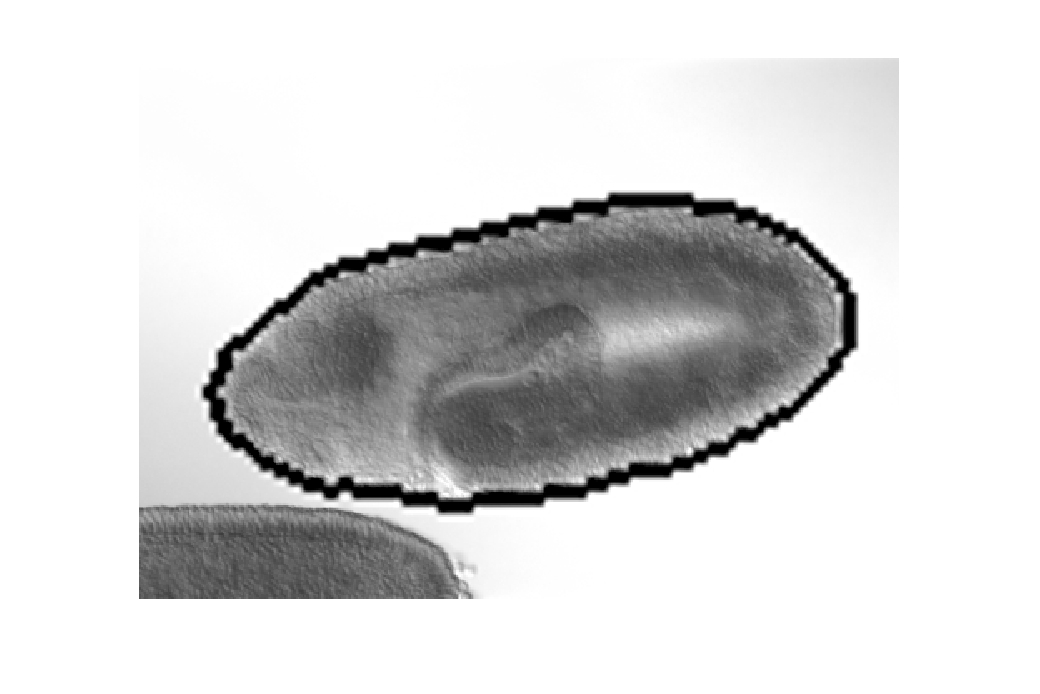
\includegraphics[scale=0.25]{hybridPriorTouching4.pdf}
}
\subfigure{
  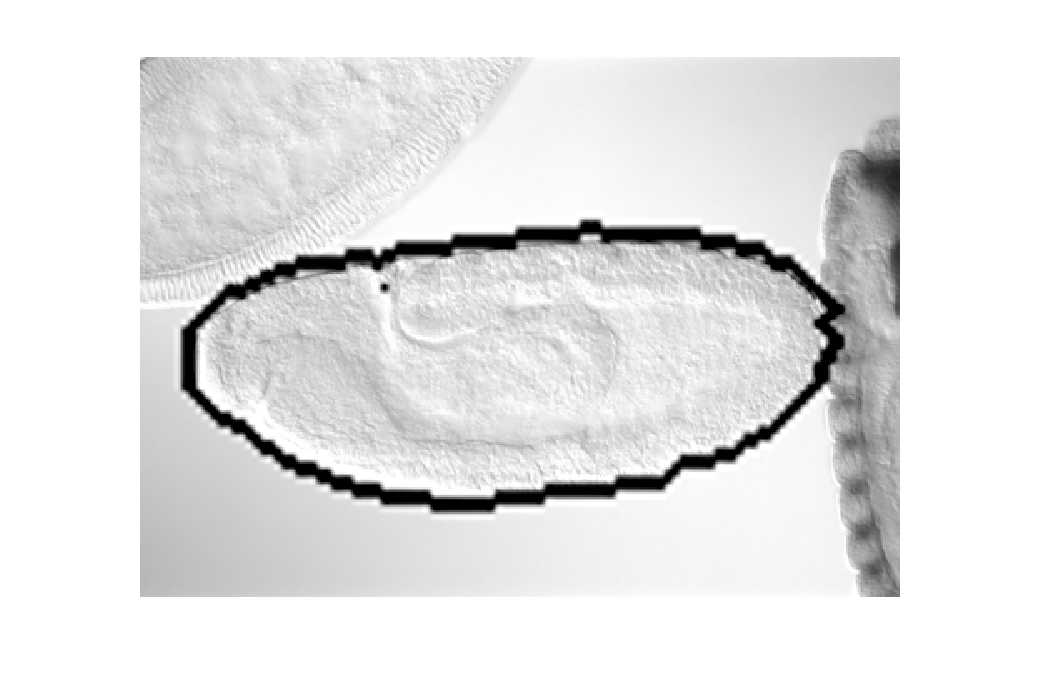
\includegraphics[scale=0.25]{hybridPriorTouching6.pdf}
}
\subfigure{
  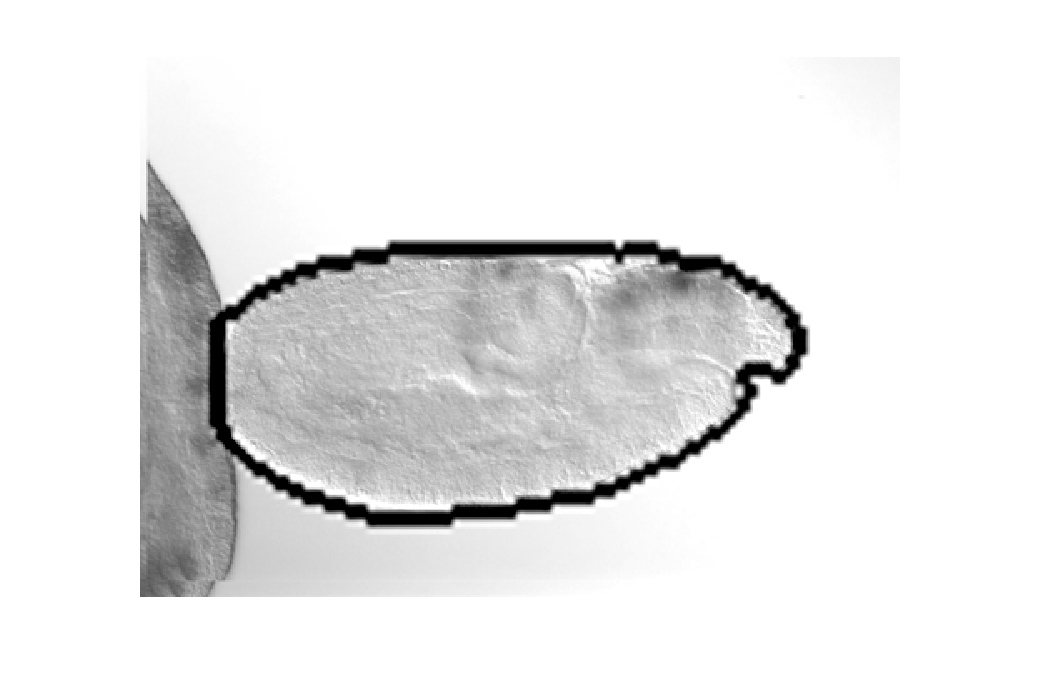
\includegraphics[scale=0.25]{hybridPriorTouching7.pdf}
}
\subfigure{
  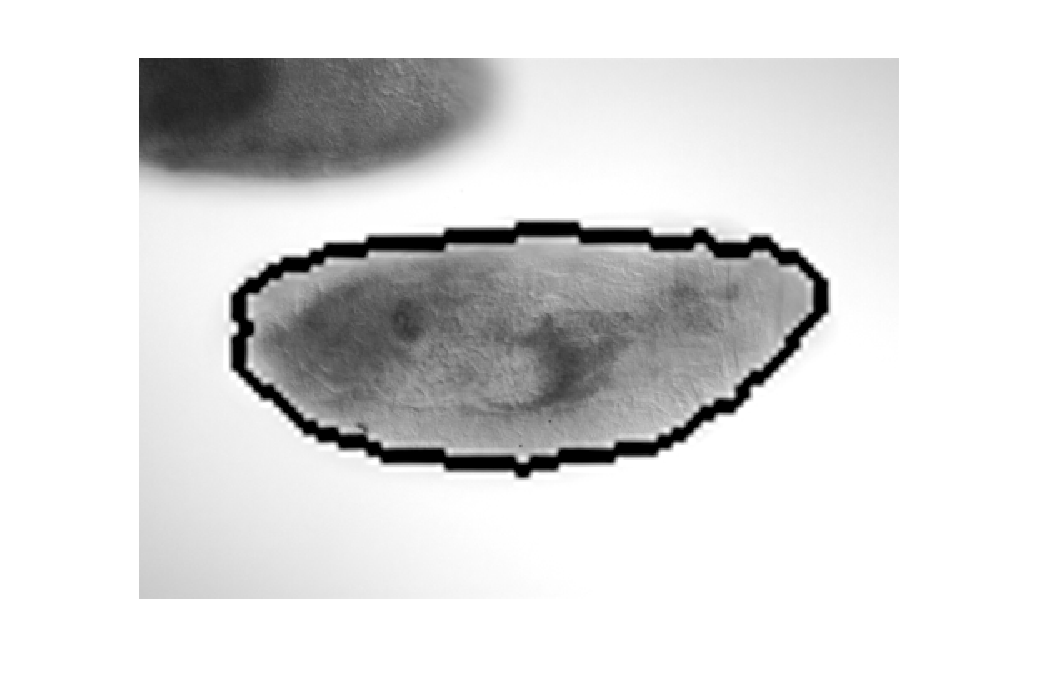
\includegraphics[scale=0.25]{hybridPriorTouching8.pdf}
}
\subfigure{
  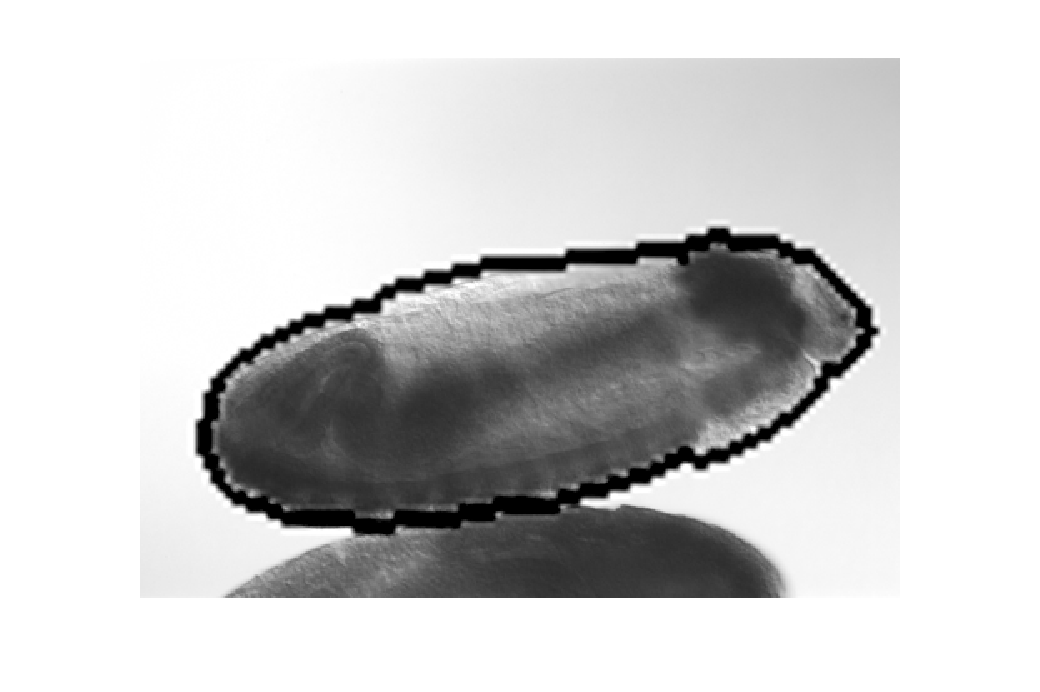
\includegraphics[scale=0.25]{hybridPriorTouching9.pdf}
}
\subfigure{
  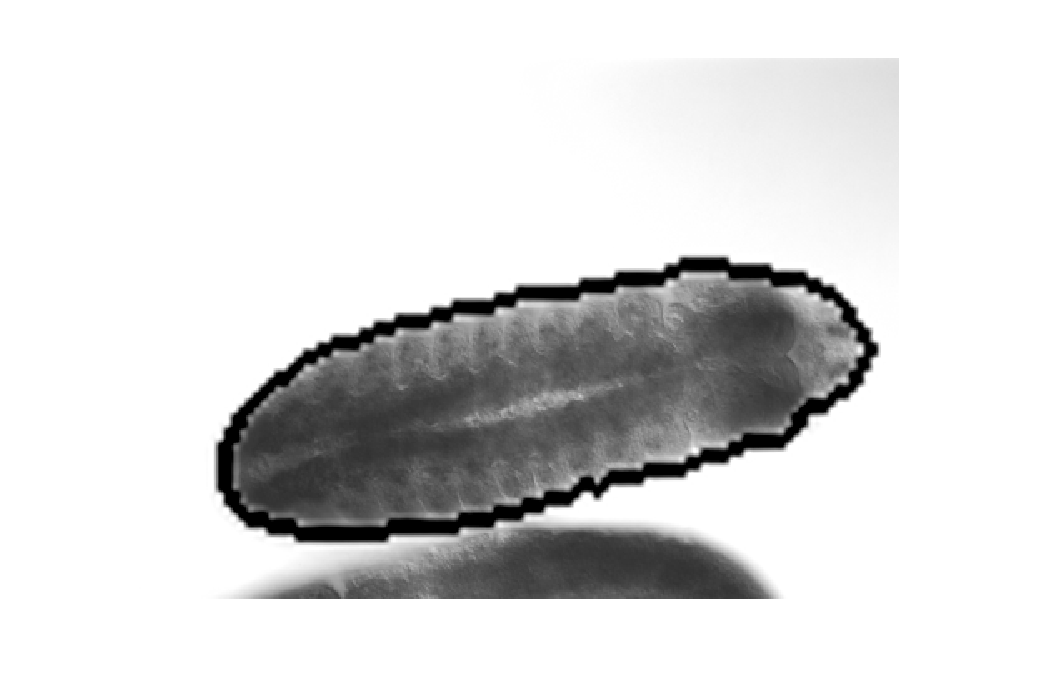
\includegraphics[scale=0.25]{hybridPriorTouching11.pdf}
}
\caption{Segmentation results on 6 different test embryos}
\label{ResultsTest}
\end{figure}

Figure \ref{Iterations} shows in detail how the algorithm evolves over the iteration steps. In the first iteration the MRF selects parts of the picture with relatively darker intensity and high standard deviation. This particularly includes the half-embryo which sticks in from the right. After one iteration of the level set segmentation with prior we see that it focuses the attention to the center and away from the very strong intensity cue on the right. The MRF then incorporates this new information while joint effort of prior and intensity cues from the superpixel MRF pushes the contour to the boundary of the embryo until it converges.

\begin{figure}[htbp]
\centering
\subfigure[]{
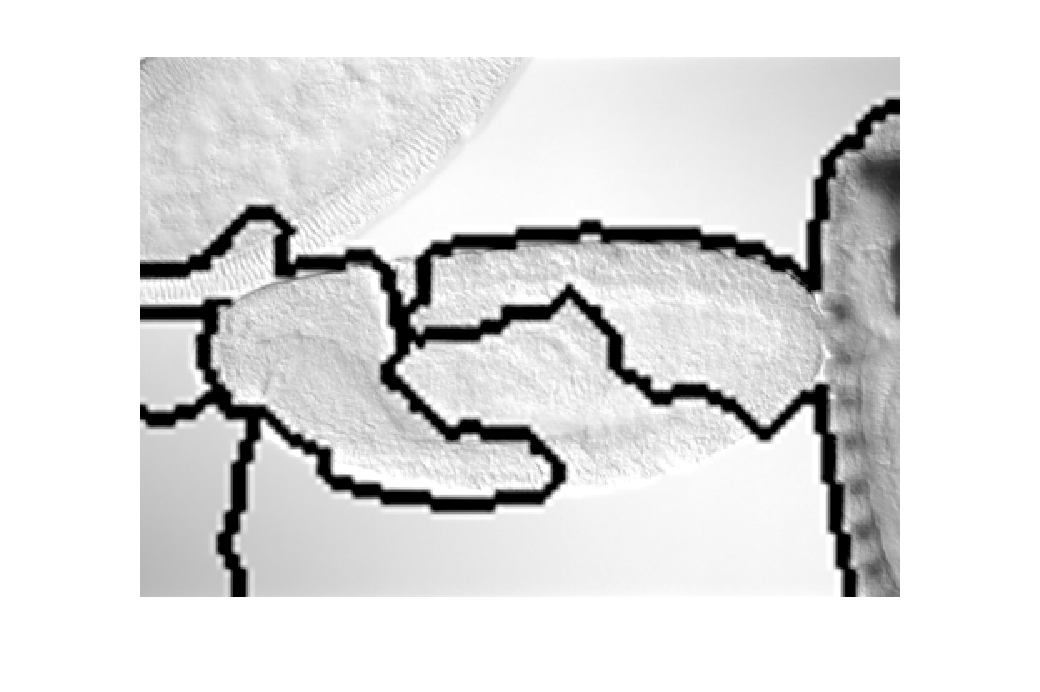
\includegraphics[scale=0.3]{hPT6_MRF1.pdf}
}
\subfigure[]{
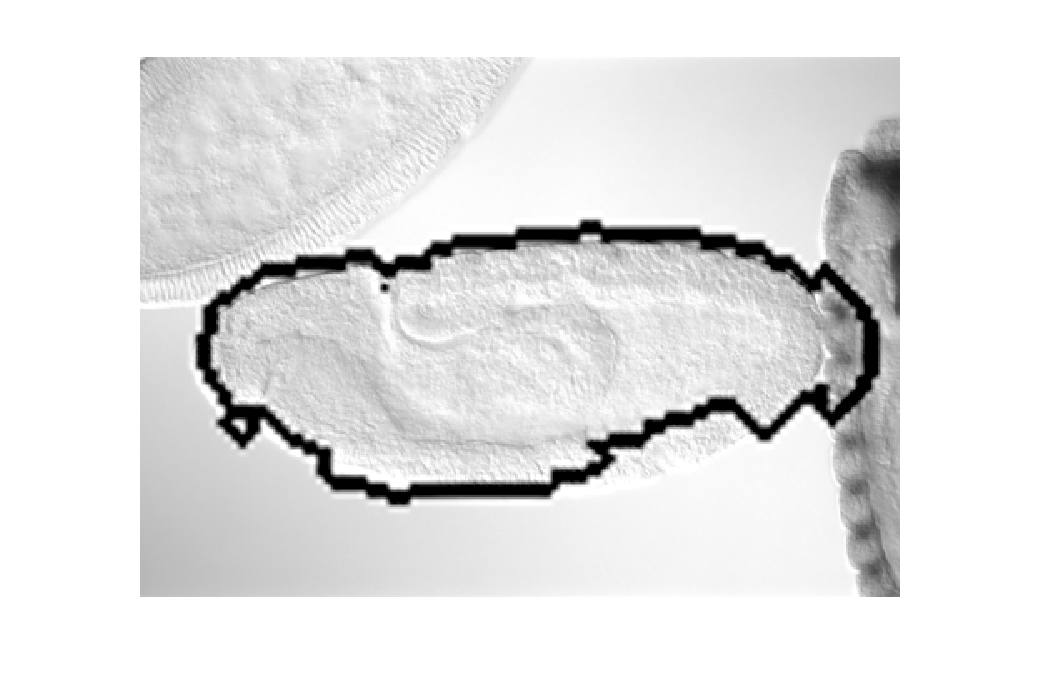
\includegraphics[scale=0.3]{hPT6_CV1.pdf}
}
\subfigure[]{
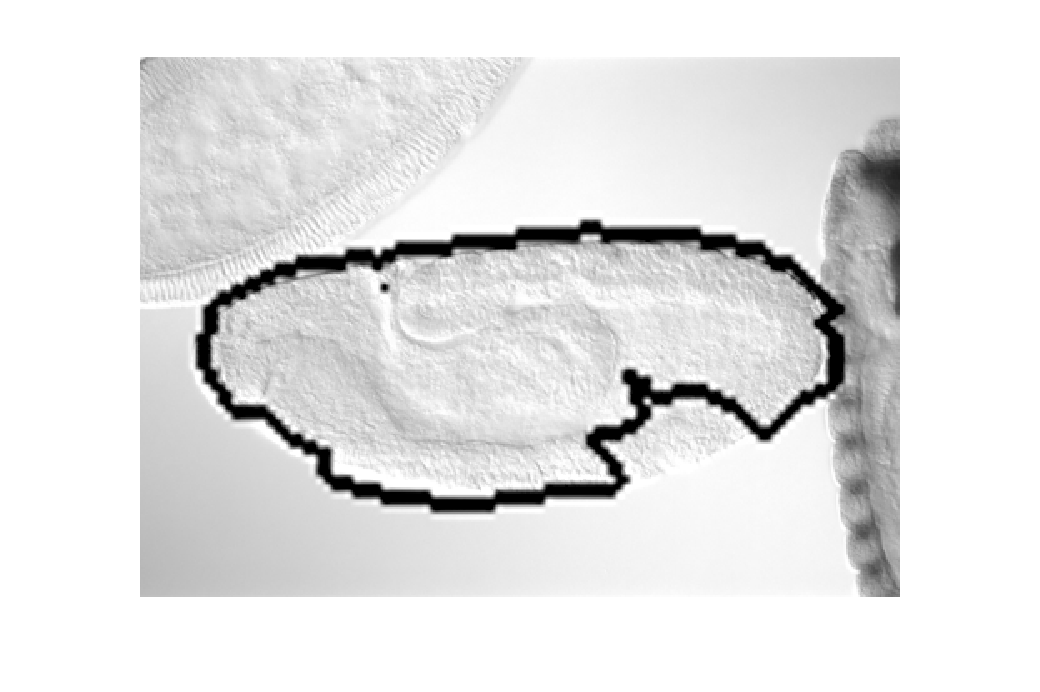
\includegraphics[scale=0.3]{hPT6_MRF2.pdf}
}
\subfigure[]{
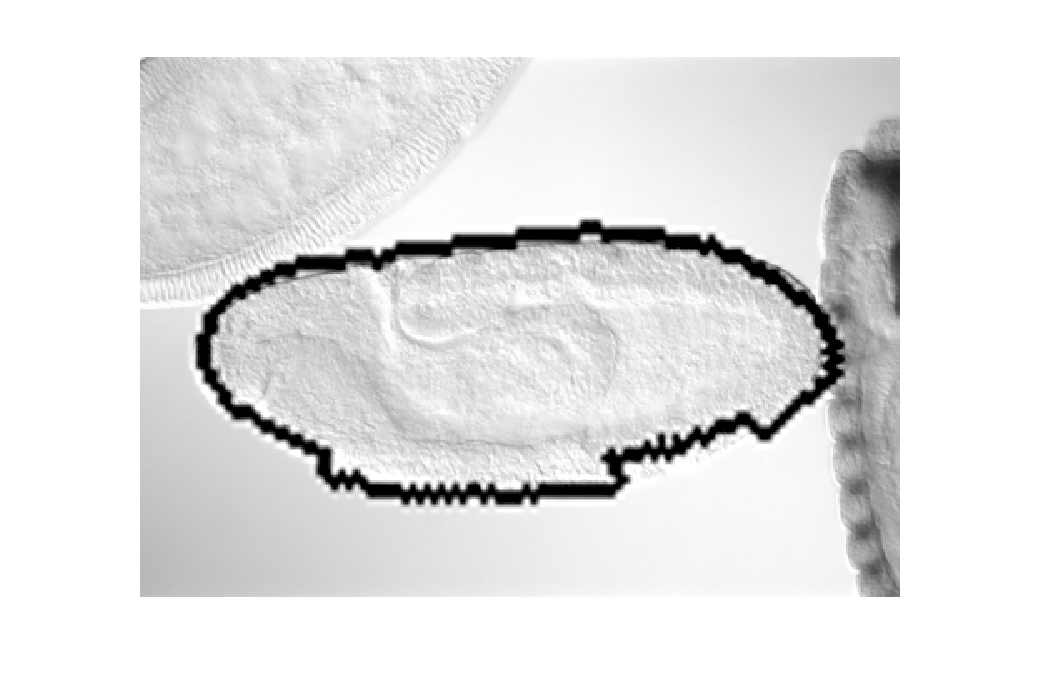
\includegraphics[scale=0.3]{hPT6_CV2.pdf}
}
\subfigure[]{
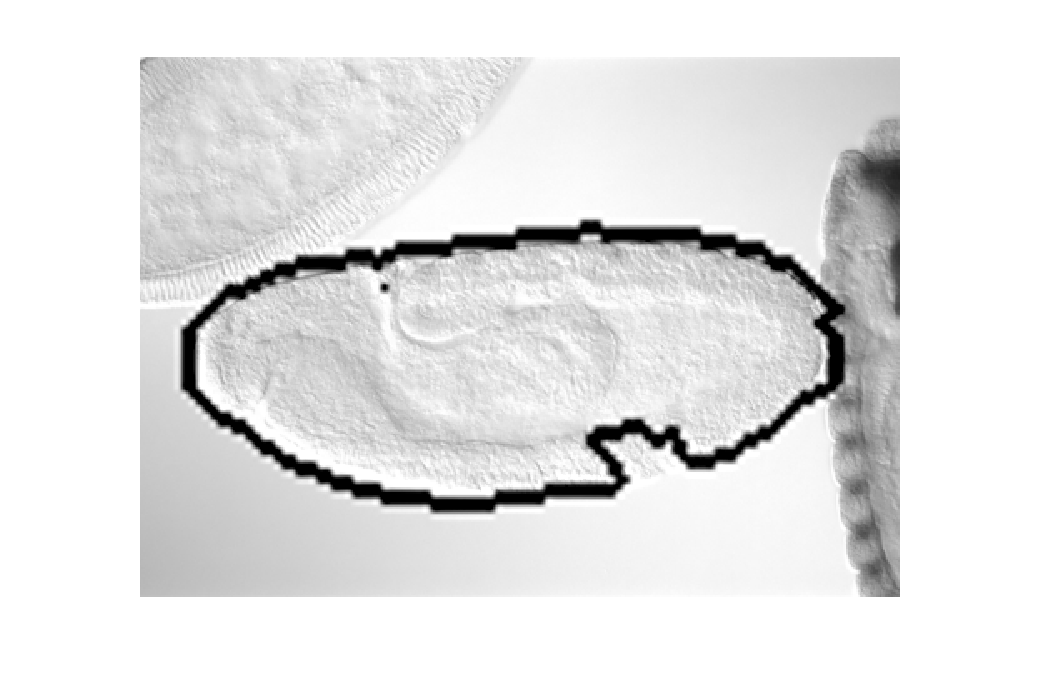
\includegraphics[scale=0.3]{hPT6_MRF3.pdf}
}
\subfigure[]{
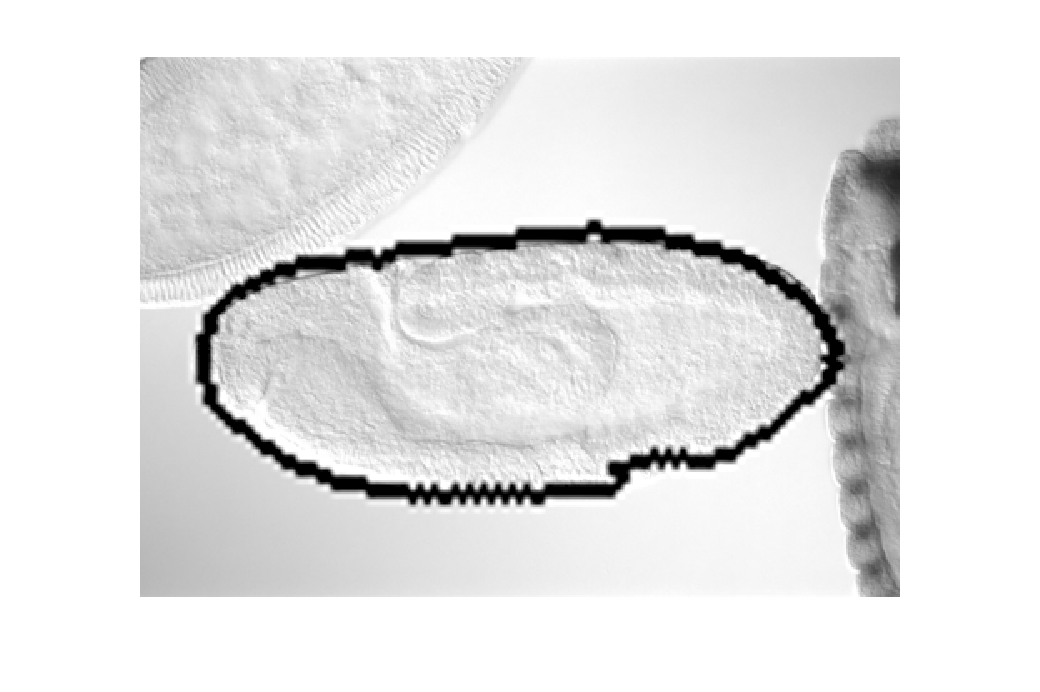
\includegraphics[scale=0.3]{hPT6_CV3.pdf}
}
\subfigure[]{
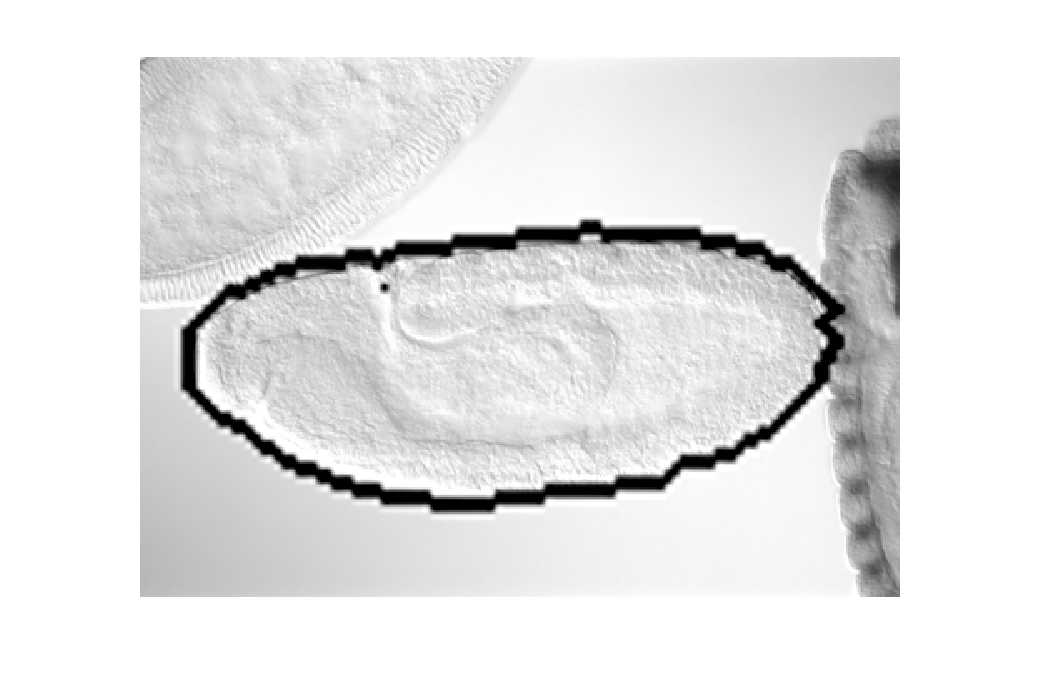
\includegraphics[scale=0.3]{hPT6_MRF4.pdf}
}
\subfigure[]{
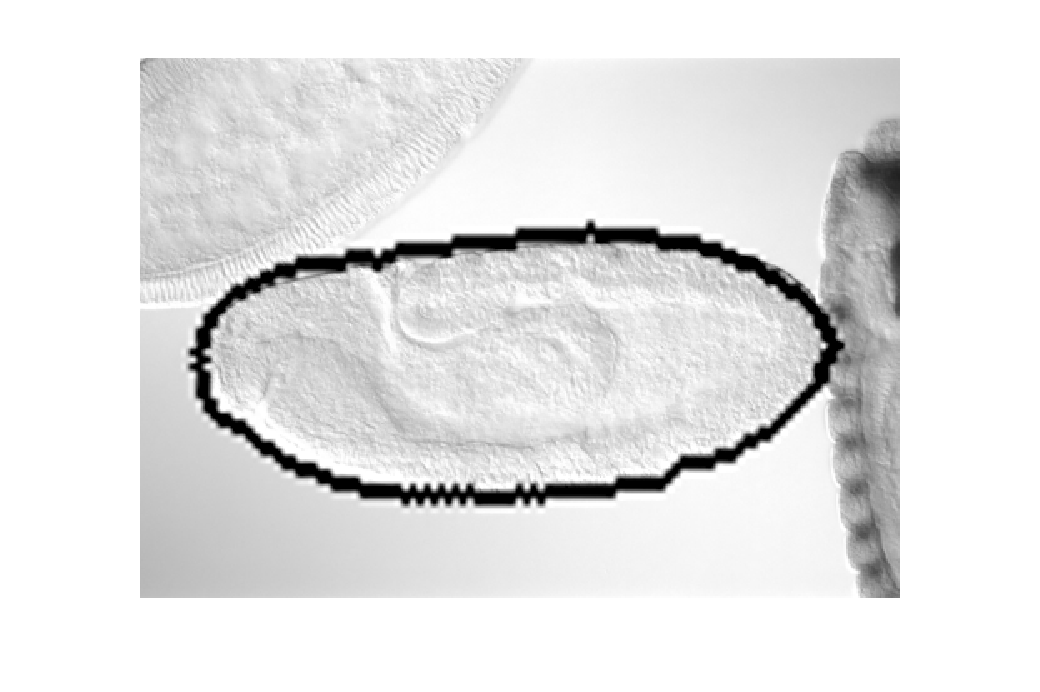
\includegraphics[scale=0.3]{hPT6_CV4.pdf}
}
\caption{This series of pictures depicts the algorithm at different iteration steps for one image. Each row corresponds to one iteration where the left column depicts the MRF result and the right column depicts the level set segmentation result}
\label{Iterations}
\end{figure}



\section{Summary and Outlook}
We have proposed an algorithm combining the advantages of the Markov Random Field model applied on superpixel features, and the level set segmentation framework which allows an easy way to incorporate shape priors. It shows very accurate behavior in the segmentation of touching embryos for which the edge and intensity cues alone are not enough for correct segmentation. 

The next step would be to test it on the actual data set for the segmentation of the gut. Preliminary results looked quite encouraging, but have to be validated on more data. The ultimate goal of simultaneous organ segmentation could then be tackled by providing a multilabel extension to this framework which works for $K=2$ (because of the single level set function).

Given enough training data, it should also be possible to train the parameters $\mu, \sigma, \theta$  beforehand so that the EM iteration can be boiled down to the E-Step alone, which is equivalent to the mean field approximation for the marginal $Q_M(y_i|x,a)$.

Furthermore it would be desirable to have a better feature set for which the Markov Random Field already gives better initial results to speed up the runtime of the algorithm. As a minor point we also need to find good stopping conditions for the level set part.

Last but not least it would be interesting to compare the performance of our hybrid model to the work in \cite{Huang04_MRFDM}, \cite{Schlesinger13}.

\section{Acknowledgements}
I want to particularly thank Siqi Wu for his support, introducing me to the problem and helping out on the implementation part. I also want to thank Antony Joseph, Zac Zhang and Erwin Frise for valuable discussions on various results and problems which occurred using previous segmentation algorithms on this data set.

\FloatBarrier
\vskip 0.2in
%\nocite{*}
\bibliographystyle{plain}
\bibliography{lit}

\end{document}
